\documentclass[tikz,border=12pt]{standalone}
\usepackage[T1]{fontenc}
\usepackage{mathpazo}
\usepackage{amsmath,amssymb}
\usetikzlibrary{arrows.meta, positioning, calc, fit, decorations.pathreplacing}

\definecolor{stblue}{HTML}{7B97AD}
\definecolor{rwgold}{HTML}{B8995E}
\definecolor{sage}{HTML}{7A9A7E}
\definecolor{dkbrown}{HTML}{3D3530}
\definecolor{wmgray}{HTML}{7B7067}
\definecolor{cream}{HTML}{F9F6F0}
\definecolor{border}{HTML}{D4C9B8}
\definecolor{terracotta}{HTML}{C47A6A}
\definecolor{lavender}{HTML}{907EA0}

\begin{document}
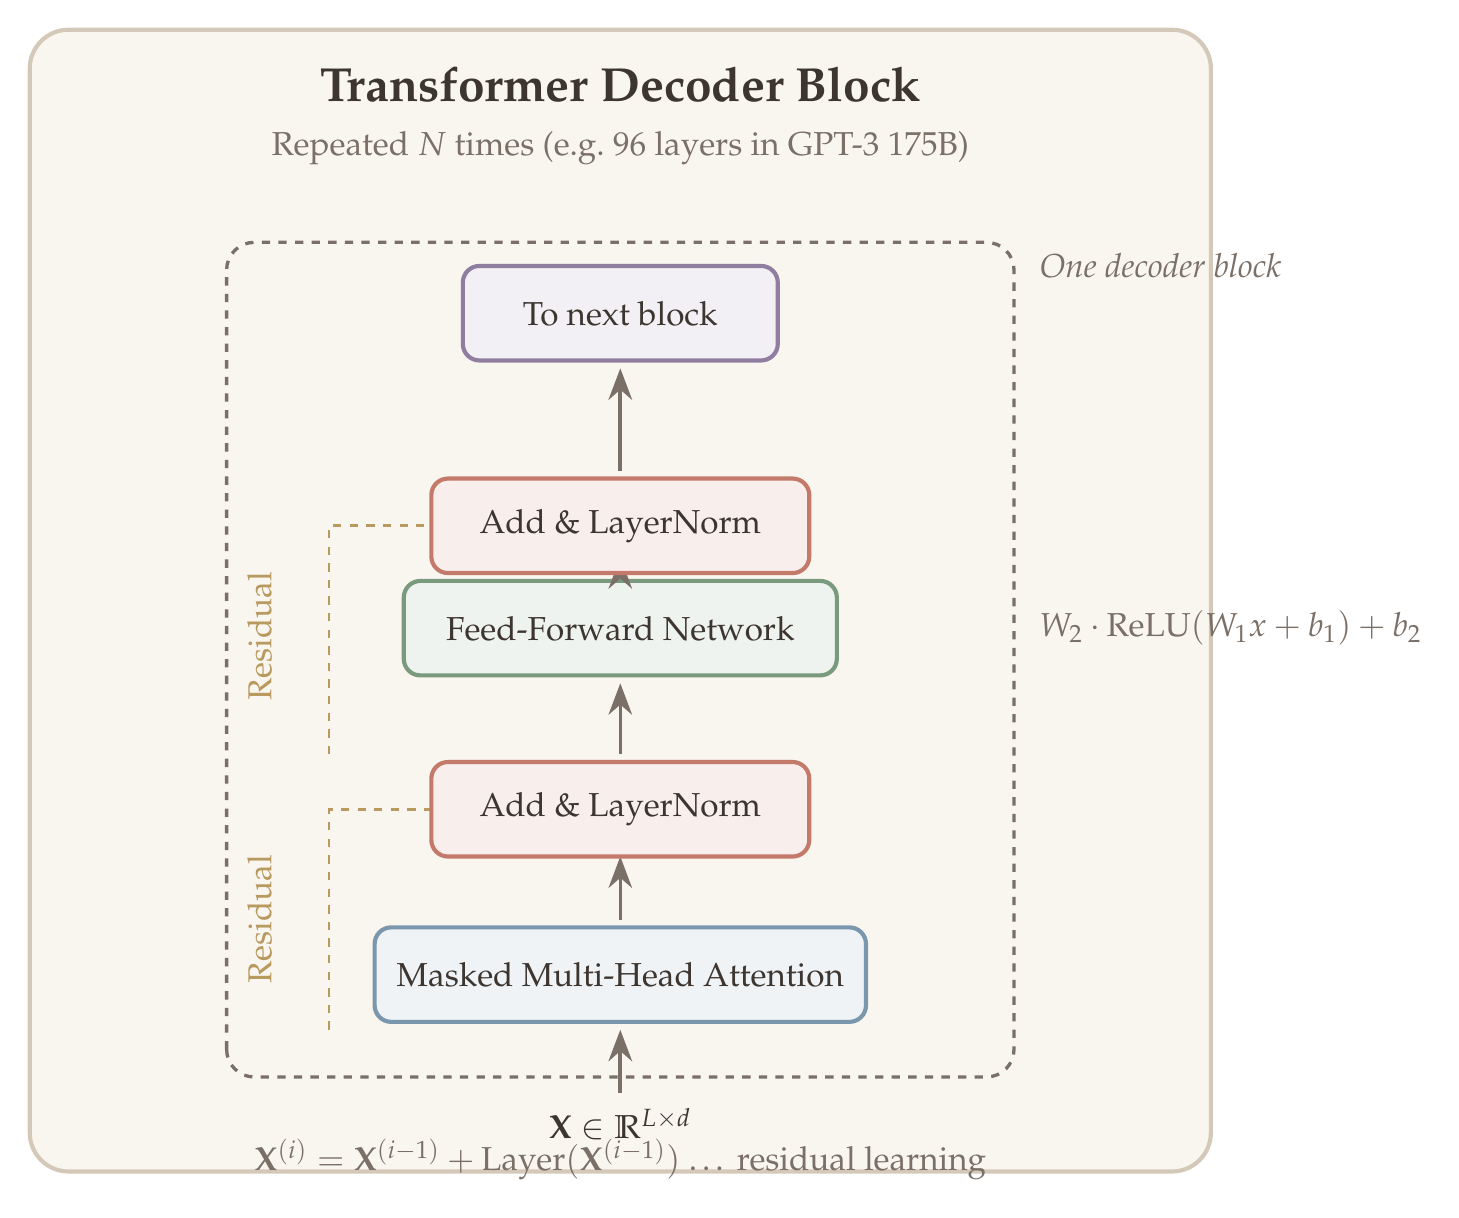
\begin{tikzpicture}[
  >={Stealth[length=4mm, width=3mm]},
  every node/.style={text=dkbrown, font=\large},
  block/.style={rounded corners=6pt, line width=1.5pt, minimum height=1.2cm, minimum width=5.5cm, align=center, inner sep=8pt},
]

% Background
\fill[cream, rounded corners=14pt] (0,0) rectangle (15,14.5);
\draw[border, line width=1.5pt, rounded corners=14pt] (0,0) rectangle (15,14.5);

% Title
\node[font=\LARGE\bfseries, text=dkbrown] at (7.5,13.8) {Transformer Decoder Block};
\node[font=\large, text=wmgray] at (7.5,13.0) {Repeated $N$ times (e.g.\ 96 layers in GPT-3 175B)};

% Dashed bounding box for one block
\draw[wmgray, line width=1.2pt, rounded corners=10pt, dashed]
  (2.5,1.2) rectangle (12.5,11.8);
\node[font=\large\itshape, text=wmgray, anchor=west] at (12.7,11.5) {One decoder block};

% Input at bottom
\node[font=\large] at (7.5,0.6) {$\mathbf{X} \in \mathbb{R}^{L \times d}$};
\draw[wmgray, line width=1.5pt, ->] (7.5,1.0) -- (7.5,1.8);

% Masked Multi-Head Self-Attention
\node[block, fill=stblue!12, draw=stblue] (mha) at (7.5,2.5) {Masked Multi-Head Attention};

% Residual connection 1 (bypass on left)
\draw[rwgold, line width=1pt, dashed]
  (3.8,1.8) -- (3.8,4.6) -- (5.5,4.6);
\node[font=\large, text=rwgold, rotate=90, anchor=south] at (3.2,3.2) {Residual};

% Plus circle
\node[circle, draw=rwgold, line width=0.8pt, fill=rwgold!15, inner sep=2pt, font=\large\bfseries, text=rwgold] (plus1) at (5.8,4.6) {$+$};

% Arrow from MHA up
\draw[wmgray, line width=1pt, ->] (7.5,3.2) -- (7.5,4.0);

% Add & LayerNorm 1
\node[block, fill=terracotta!12, draw=terracotta, minimum width=4.8cm] (an1) at (7.5,4.6) {Add \& LayerNorm};

% Arrow to FFN
\draw[wmgray, line width=1pt, ->] (7.5,5.3) -- (7.5,6.2);

% Feed-Forward Network
\node[block, fill=sage!12, draw=sage] (ffn) at (7.5,6.9) {Feed-Forward Network};
\node[font=\large\itshape, text=wmgray, anchor=west] at (12.7,6.9) {$W_2 \cdot \mathrm{ReLU}(W_1 x + b_1) + b_2$};

% Residual connection 2
\draw[rwgold, line width=1pt, dashed]
  (3.8,5.3) -- (3.8,8.2) -- (5.5,8.2);
\node[font=\large, text=rwgold, rotate=90, anchor=south] at (3.2,6.8) {Residual};

% Plus circle 2
\node[circle, draw=rwgold, line width=0.8pt, fill=rwgold!15, inner sep=2pt, font=\large\bfseries, text=rwgold] (plus2) at (5.8,8.2) {$+$};

% Arrow from FFN up
\draw[wmgray, line width=1pt, ->] (7.5,7.6) -- (7.5,7.8);

% Add & LayerNorm 2
\node[block, fill=terracotta!12, draw=terracotta, minimum width=4.8cm] (an2) at (7.5,8.2) {Add \& LayerNorm};

% Arrow to output
\draw[wmgray, line width=1.5pt, ->] (7.5,8.9) -- (7.5,10.2);

% To next block
\node[block, fill=lavender!12, draw=lavender, minimum width=4.0cm] (next) at (7.5,10.9) {To next block};

% Bottom note
\node[font=\large, text=wmgray] at (7.5,0.15) {$\mathbf{X}^{(i)} = \mathbf{X}^{(i-1)} + \mathrm{Layer}(\mathbf{X}^{(i-1)})$ \ldots\ residual learning};

\end{tikzpicture}
\end{document}
